\documentclass{article}

\usepackage{tikz}
\usepackage{float}
\usepackage{array}

\usetikzlibrary{arrows}
\usetikzlibrary{shapes}
\usetikzlibrary{scopes}

\title{Learning Ti\textit{k}Z}
\date{}

\setcounter{totalnumber}{4} 

\begin{document}
	\maketitle
	
	\section{Inline Graphics}
	Inline small rectangle: 
	\tikz \draw (0,0) rectangle (0.25,0.25);
	, this is a small 
	\tikz \draw (0,0) -- (0.5,0); Line
	\tikz \draw (0,0) -- (0.5,0.5); \\
	
	For multiple objects:
	\tikz{
		\draw (0,0) rectangle (0.25,0.25);
		\draw (0,0) rectangle (0.5,0.5);
		\draw (0.7,0) rectangle (0.95,0.25);
	}
	
	\vspace{0.5cm}
	Some textual content 
	\tikz{
		\draw (0,0) circle (5pt);
		\fill (0,0) circle (0.5pt);
	}
	Other textual content. \\
	
	\noindent
	Now centering the circle 
	\tikz[baseline=-2.5pt]{\draw (0,0) circle (5pt);}
	to the surrounding text.
	
	\vspace{0.5cm}
	
	\noindent The following draw is a $4 \times 2$				Crossed rectangle:
	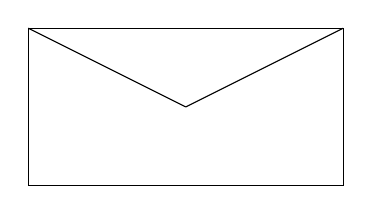
\begin{tikzpicture}
		\draw (0,0) rectangle (4,2);
		\draw (2,1) -- (4,2); % Right Line
		\draw (2,1) -- (0,2); % Left Line
	\end{tikzpicture}
	
	\subsection{Scope Environment}
	\frame{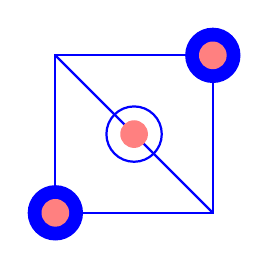
\begin{tikzpicture}
		\begin{scope}[blue, thick]
			\draw (0,0) rectangle (2,2);
			\fill (0,0) circle (10pt);
			\draw (1,1) circle (10pt);
			\draw (0,2) -- (2,0);
			\fill (2,2) circle (10pt);
		\end{scope}
		\begin{scope}[red!50]
			\fill (0,0) circle (5pt);
			\fill (1,1) circle (5pt);
			\fill (2,2) circle (5pt);
		\end{scope}
	\end{tikzpicture}}
	Some textual Content.
	
	\subsection{The Bounding Box}
	\tikz{
		\useasboundingbox (0,0) rectangle (2,2);
		\draw (0,0) rectangle (2,2);
		\fill[red] (0.5,0) -- (1.5,0) -- (1,1) 							-- (0.5,0);
		\fill[blue] (4,-0.5) circle (0.5); % def:cm
	}
	Gravity or gravitation, is a natural phenomenon by which all things with mass or energy-including planets, stars, galaxies, and even light are brought toward (or gravitate toward) one another. On Earth, gravity gives weight to physical objects, and the Moon's gravity causes the ocean tides.
	
	\section{Placing Grids}
	\tikz{
		\draw[step=0.5] (0,0) grid (2,2);	
		\fill[blue!70] (1,1) circle (3pt);
	}  
	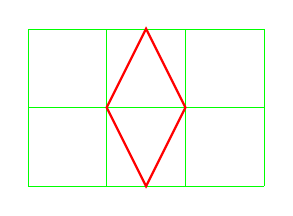
\begin{tikzpicture}
		\draw[help lines, green] (0,0) grid (3,2);
		\draw[red, thick] (1,1) -- (1.5,2) -- (2,1)
				-- (1.5,0) -- cycle;
	\end{tikzpicture}
	
	\section{Constructing Paths}
	\tikzset{help lines/.style={thin, color=green}}
	\subsection{Ti{\textit k}Z Paths} % what are paths
	Inside a tikzpicture environment everything is 				drawn by starting a path and by extending the path.
	\frame{
\begin{tikzpicture}
		\path (0,0) -- (3,0);
		% \draw = \path[draw]
		\path[draw,red,ultra thick] (1,0) -- (2,0);
		\draw[blue, ultra thick] (2.5,0) -- (4,0);
	\end{tikzpicture}}
	
	\subsection{Example on Paths}
	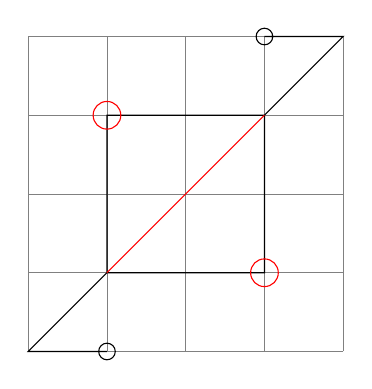
\begin{tikzpicture}
		\draw[help lines] (0,0) grid (4,4);
		\draw (1,0) circle (3pt) -- (0,0) -- (1,1) 
			rectangle (3,3) -- (4,4) -- (3,4) circle 
			(3pt);
		\path[draw, red] 
				(1,1) -- (2,2) 
				(1,3) circle (5pt) 
				(2,2) -- (3,3)
				(3,1) circle (5pt); 
	\end{tikzpicture}
	
	\subsection{Defining Coordinate Labels}
	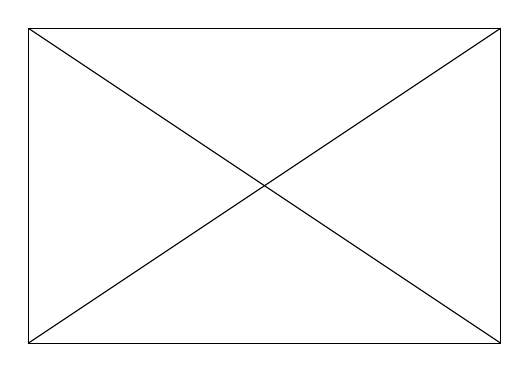
\begin{tikzpicture}
		% Defining the start-end corners of the rect.
		%	while drawing the / half-cross line
		\draw (0,0) coordinate (Lower Left) -- (6,4)
			coordinate (Upper Right);
		% Using the labels to create the rectangle
		\draw (Lower Left) rectangle (Upper Right);
		% Drawing the \ other half-cross line.
		\draw (0,4) -- (6,0);
	\end{tikzpicture}
	
	\pagebreak	
	
	\subsection{Path Extension Operations}
	
	\subsubsection{The move-to Operation}
	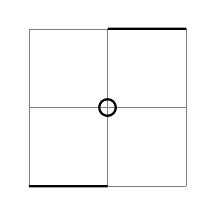
\begin{tikzpicture}
		\draw[help lines] (0,0) grid (2,2);
		\draw[thick] (0,0) -- (1,0)
					 (1,1) circle (3pt)
					 (1,2) -- (2,2);
	\end{tikzpicture}
	
	\subsubsection{The line-to Operation}
	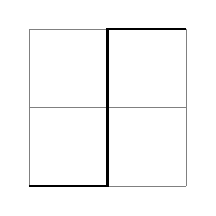
\begin{tikzpicture}
		\draw[help lines] (0,0) grid (2,2);
		\draw[thick] (0,0) -- (1,0) --
		             (1,2) -- (2,2);
	\end{tikzpicture}
	
	\subsubsection{The curve-to Operation}
	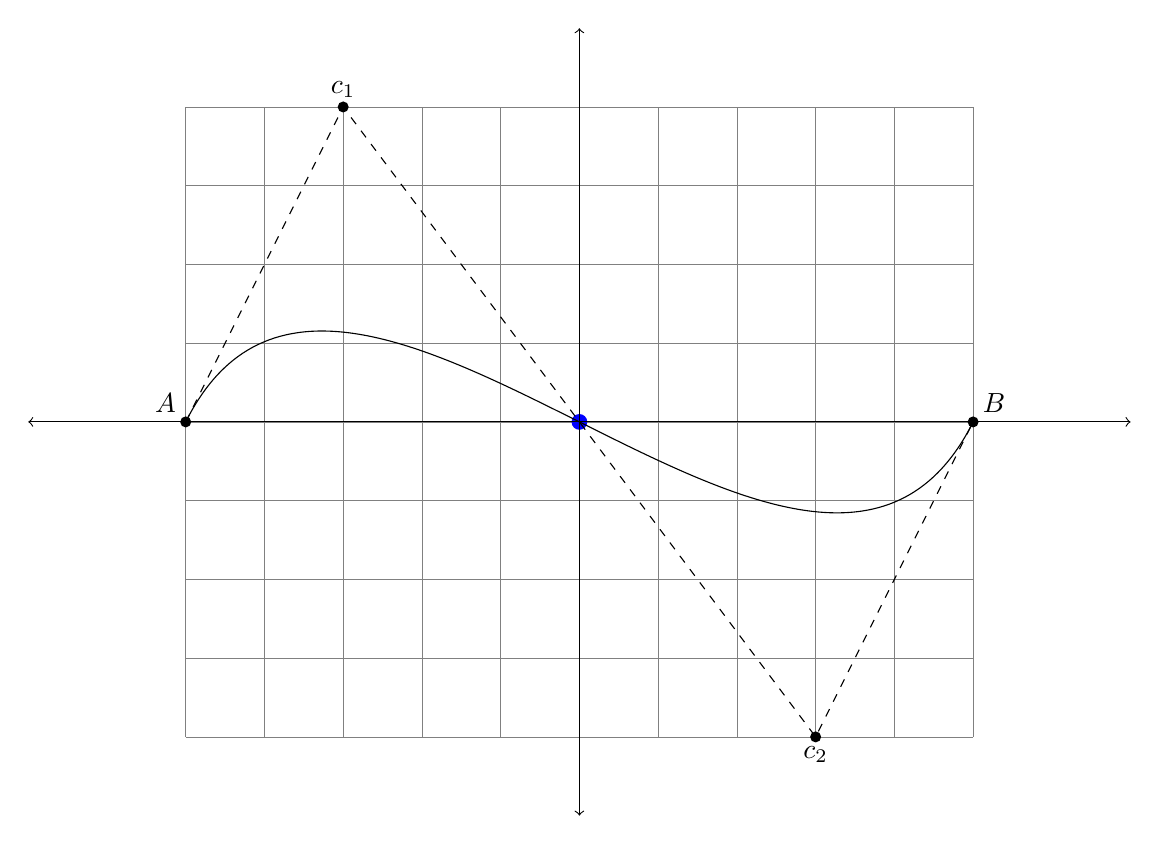
\begin{tikzpicture}
		\draw[help lines] (-5,-4) grid (5,4);
		\fill[blue] (0,0) coordinate (o) 
							circle (0.1);
		%% The Axes
		\draw[<->] (-7,0) -- (7,0); % x-axis 
		\draw[<->] (0,-5) -- (0,5); % y-axis
		%% Invisibly Defining the Labels for Coords
		\path 
			(-5,0) coordinate (p_st)
			(-3,4) coordinate (c1)
			(3,-4) coordinate (c2)
			(5,0)  coordinate (p_en);
		%% fill-drawing the points
		\fill 
			 (p_st) circle (0.7mm) % Start Point
			 (c1)   circle (0.7mm) % Control Point1
			 (c2)   circle (0.7mm) % Control Point2
			 (p_en) circle (0.7mm);% End Point
		% Drawing the curve
		\draw (p_st) .. controls (c1) and (c2) ..
				 (p_en);
		%% Connecting with a dashed line
		\draw[dashed] (p_st) -- (c1) -- (c2) -- (p_en);
		%% Using Nodes for Labeling
		\draw (p_st) node[anchor=south east] {$A$}
			  (c1) node[anchor=south] {$c_1$}
			  (c2) node[anchor=north] {$c_2$}
			  (p_en) node[anchor=south west] {$B$};
			  
	\end{tikzpicture}
	
	\subsubsection{The cycle Operation}
	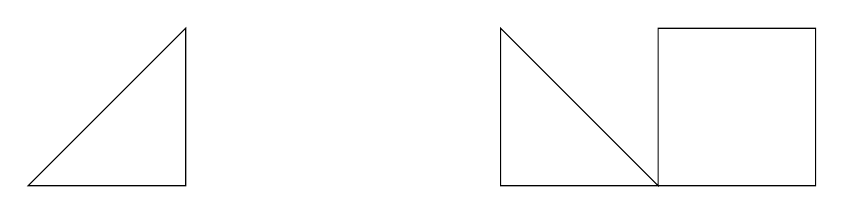
\begin{tikzpicture}
		\draw (0,0) -- (2,0) -- (2,2) -- cycle;
		\draw (6,2) -- (6,0) -- (10,0) -- (10,2)
				-- (8,2) -- (8,0) -- cycle;
	\end{tikzpicture}
	
	\subsubsection{The Double line-to Operations}
	\setlength\extrarowheight{3pt}
	\begin{tabular}{|c|c|}
		\hline
		Horizontal followed by Vertical &
		Vertical followed by Horizontal \\
		\hline
		\begin{tikzpicture}
			\path (0,0) rectangle (6,4.25);
			\fill (0,0) circle (0.1)
				  (6,4) circle (0.1);
			\draw (0,0) -| (6,4);
		\end{tikzpicture}
		& 
		\begin{tikzpicture}
			\fill (0,0) circle (0.1)
				  (6,4) circle (0.1);
			\draw (0,0) |- (6,4);
		\end{tikzpicture} \\
		\hline
	\end{tabular}
	
	\subsubsection{The rectangle Operation}
	
\begin{tikzpicture}
		\fill (0,0) rectangle (3,1) rectangle (6,2)
				(6,1) rectangle (9,0);
	\end{tikzpicture}
	
	\subsubsection{The arc and ellipse Operations}
	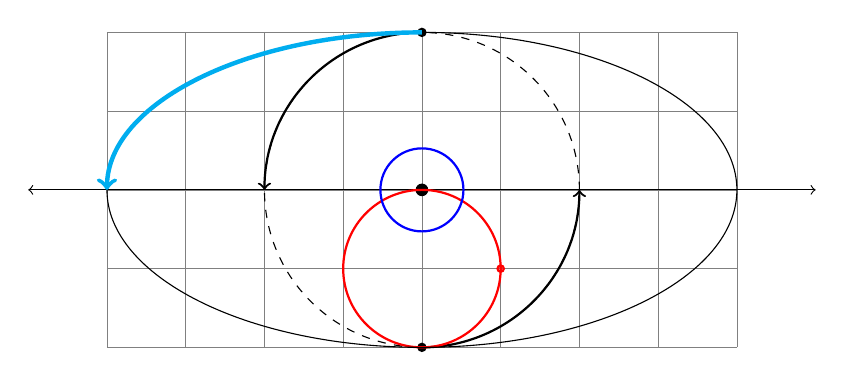
\begin{tikzpicture}
		\draw[help lines] (0,0) grid (8,4);
		\draw[<->] (-1,2) -- (9,2);
		%% The Arcs
		\draw[dashed] (4,2) circle (2);
		\fill 
			(4,2) circle (0.8mm)
			(4,4) coordinate (p1) circle (0.6mm)
			(4,0) coordinate (p2) circle (0.6mm);
		\draw[->, thick] (p1) arc (90:180:2cm);
		\draw[->, thick] (p2) arc (-90:0:2cm);
		% 0 isn't 360 
		\draw[thick, red] (5,1) circle (0.4mm)
					(5,1) arc (0:360:1cm);
		%% The Ellipse
		\draw (4,2) ellipse (4cm and 2cm);
		\draw[thick,blue] (4,2) ellipse (15pt and 15pt);
		%% The Elliptical Arc
		\draw[->,cyan,ultra thick] (p1) 
				arc (90:180:4cm and 2cm);
	\end{tikzpicture}
	
	%%%%%%%%%%%%%%%%%%%%%%%%%%%%%%%%%%%%%%%%%%%%%%%%%
 	%%%%%%%%%%%%%%%%%%%%%%%%%%%%%%%%%%%%%%%%%%%%%%%%%
 	
 	\pagebreak
 	
 	\subsection{Styling Paths}
 	
 	\subsubsection{Filling Paths}
 	\tikz \fill[blue] (0,0) circle (1);
 	\hspace{1cm}
 	\tikz \filldraw[ultra thick, fill=gray, draw=black] 
 		(0,0) rectangle (2,2);
 	
 	\subsubsection{Shading Paths}
 	Shading Commands must be Inserted inside a					tikzpicture environment. \\
 	
\begin{tikzpicture}
 		\shade[left color=cyan, right color=green]  
 			(0,0) rectangle (6,2);
 		\shade[left color=red!70, right color=blue!80]
 			(8,1) circle (1);
 	\end{tikzpicture} \\ 
 	
 	\vspace{-5pt}
 	
 	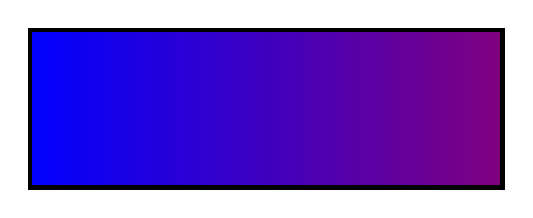
\begin{tikzpicture}[ultra thick]
 		\shadedraw[left color=blue, right color=violet,
 			draw=black]
 			(0,0) rectangle (6,2);
 	\end{tikzpicture}
 	
 	\subsubsection{Coloring Paths}
 	
\begin{tikzpicture}[color=teal, ultra thick]
 		\draw (0,0) -- (3,0) -- (3,3) -- cycle;
 		\draw (4,1.5) circle (20pt);
 		\draw[olive] (5,0) rectangle (10,3); 
 	\end{tikzpicture}
 	
 	\subsubsection{Setting the Line Width}
 	% default is "thin" = 0.4pt
 	
\begin{tikzpicture}
 		\draw[line width=5pt] (0,2) -- (0,0) -- 
 			(4,2) -- (4,0) -- cycle; 
 	\end{tikzpicture}
 	
 	\pagebreak
 	
 	\subsubsection{Line Caps and Joins}
 	\begin{tabular}{|c|c|}
 		\hline
 		\textbf{Line Caps} & \textbf{Line Joins} \\
 		\hline
 		round, rect, and butt & 
 				round, bevel, and miter \\
 		\hline
 		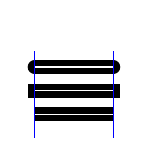
\begin{tikzpicture}[line width=5pt]
 			\path (0,3) -- (0,3.5);
 			\draw[line cap=round] (0,3) -- (1,3);
 			\draw[line cap=rect]  (0,2.7) -- (1,2.7);
 			\draw[line cap=butt]  (0,2.4) -- (1,2.4);
 			\draw[white,line width=0.5pt]
 					(0,3) 	-- (1,3)
 					(0,2.7) -- (1,2.7)
 					(0,2.4) -- (1,2.4);
 			% The Extra space to the right and left 
 			%    of the lines may add an illusion 
 			%	  that the line is expanded so:
 			\draw[blue, line width=0.5pt]
 					(0,3.2) -- (0,2.1)
 					(1,3.2) -- (1,2.1);
 		\end{tikzpicture}
 		& 
 		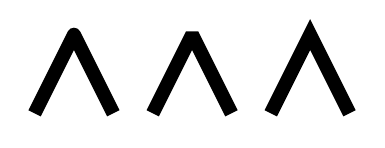
\begin{tikzpicture}[line width=5pt]
 			\draw[line join = round] (0,0) -- 
 				(0.5,1) -- (1,0);
 			\draw[line join = bevel] 
 				 	(1.5,0) -- (2,1) -- (2.5,0);
 			\draw[line join = miter] % def
 				 	(3,0) -- (3.5,1) -- (4,0);
 		\end{tikzpicture} \\
 		\hline
 	\end{tabular}
 	
 	%% Arrows
 	\subsubsection{Arrows}
 	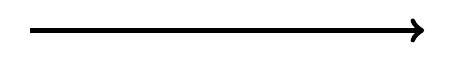
\begin{tikzpicture}[line width=2pt]
 		\draw[->] (0,0) -- (5,0);
 	\end{tikzpicture} \\
 	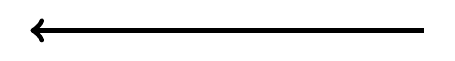
\begin{tikzpicture}[line width=2pt]
 		\draw[<-] (0,0) -- (5,0);
 	\end{tikzpicture} \\
 	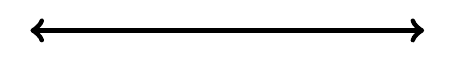
\begin{tikzpicture}[line width=2pt]
 		\draw[<->] (0,0) -- (5,0);
 	\end{tikzpicture} 
 	
 	\vspace{1cm}
 	
 	\noindent {\bf
 	\Large Changing the Arrow Head using \verb|>|= \\}
 	% \draw[define(>="style"), use(<->)]
 	\begin{tabular}{|c|c|}
 		\hline
 		\textbf{Style} & \textbf{Arrow Shape} \\
 		\hline
 		Stealth & \begin{tikzpicture}
 					\draw[>=stealth, ->] (0,0) -- (3,0);
 				  \end{tikzpicture} \\
 		Reversed& \begin{tikzpicture}
 					\draw[>=stealth reversed,->] 
 						(0,0) -- (3,0);
 				  \end{tikzpicture} \\
 		\hline
 		to [def]& \begin{tikzpicture}
 					\draw[>=to,->] (0,0) -- (3,0);
 				  \end{tikzpicture} \\
 		Reversed& \begin{tikzpicture}
 					\draw[>=to reversed,->] 
 						(0,0) -- (3,0);
 				  \end{tikzpicture} \\
 		\hline
 		latex   & \begin{tikzpicture}
 					\draw[>=latex,->] (0,0) -- (3,0);
 				  \end{tikzpicture} \\
 		Reversed& \begin{tikzpicture}
 					\draw[>=latex reversed,->] 
 							(0,0) -- (3,0);
 				  \end{tikzpicture} \\
 		\hline
 	\end{tabular}
 	
 	\vspace{1cm}
 	{\bf \Large \noindent
 	Arrow Heads within \textit{arrows} tikzlibrary}
 	
 	\begin{table}[h]
 		%% First Table
	 	\begin{tabular}{|cc|}
	 		\hline
	 		open triangle 90 &
	 		\begin{tikzpicture}
	 			\draw[>=open triangle 90, ->]
	 					(0,0) -- (3,0);
	 		\end{tikzpicture} \\
	 		open triangle 60 &
	 		\begin{tikzpicture}
	 			\draw[>=open triangle 60, ->]
	 					(0,0) -- (3,0);
	 		\end{tikzpicture} \\
	 		open triangle 45 &
	 		\begin{tikzpicture}
	 			\draw[>=open triangle 45, ->]
	 					(0,0) -- (3,0);
	 		\end{tikzpicture} \\
	 		\hline
	 	\end{tabular}
	 	%% Second Table
	 	\begin{tabular}{|cc|} %% notice the shortcut
	 		\hline
	 		triangle 90 &
	 		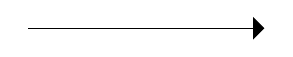
\begin{tikzpicture}
	 			\draw[-triangle 90]
	 					(0,0) -- (3,0);
	 		\end{tikzpicture} \\
	 		triangle 60 &
	 		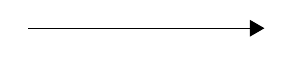
\begin{tikzpicture}
	 			\draw[-triangle 60]
	 					(0,0) -- (3,0);
	 		\end{tikzpicture} \\
	 		triangle 45 &
	 		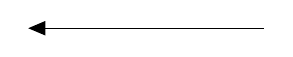
\begin{tikzpicture}
	 			\draw[triangle 45-]
	 					(0,0) -- (3,0);
	 		\end{tikzpicture} \\
	 		\hline
	 	\end{tabular}
	 	
	 	\centering
 	
		\vspace{0.4cm} 	
		
		%% Third Table
	 	\begin{tabular}{|cc|}
	 		\hline
	 		angle 90 &
	 		\begin{tikzpicture}
	 			\draw[-angle 90]
	 					(0,0) -- (3,0);
	 		\end{tikzpicture} \\
	 		angle 60 &
	 		\begin{tikzpicture}
	 			\draw[-angle 60]
	 					(0,0) -- (3,0);
	 		\end{tikzpicture} \\
	 		angle 45 &
	 		\begin{tikzpicture}
	 			\draw[-angle 45]
	 					(0,0) -- (3,0);
	 		\end{tikzpicture} \\
	 		\hline
	 	\end{tabular} \\
 		
 		
		\vspace{0.4cm} 	
	 	
	 	%% Fourth Table
	 	\begin{tabular}{|c|c|c|}
	 		\hline
	 		open diamond\,
	 		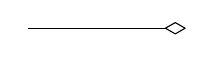
\begin{tikzpicture}
	 			\draw[-open diamond]
	 					(0,0) -- (2,0);
	 		\end{tikzpicture} &
	 		diamond\,
	 		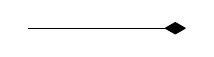
\begin{tikzpicture}
	 			\draw[-diamond]
	 					(0,0) -- (2,0);
	 		\end{tikzpicture} &
	 		o\,
	 		\begin{tikzpicture}
	 			\draw[-o]
	 					(0,0) -- (2,0);
	 		\end{tikzpicture} \\
	 		%% Second Row
	 		open square\,
	 		\begin{tikzpicture}
	 			\draw[-open square]
	 					(0,0) -- (2,0);
	 		\end{tikzpicture} &
	 		square\,
	 		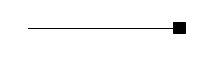
\begin{tikzpicture}
	 			\draw[-square]
	 					(0,0) -- (2,0);
	 		\end{tikzpicture} &
	 		*\,
	 		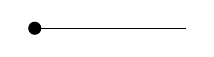
\begin{tikzpicture}
	 			\draw[*-]
	 					(0,0) -- (2,0);
	 		\end{tikzpicture} \\
	 		\hline
	 	\end{tabular}
 	\end{table}
 	
 	%%%%%%%%%%%%%%%%%%%%%%%%%%%%%%%%%%%%%%%%%%%%%%%%%
 	%%%%%%%%%%%%%%%%%%%%%%%%%%%%%%%%%%%%%%%%%%%%%%%%%
 	
 	\section{Nodes}
 	So far we've been working with drawings that
 	don't incorporate text or math or other form of
 	content, and \textit{the node operation} is the 
 	gateway to do so in tikz.
 	
 	\vspace{0.25cm}
 	
 	% \path node(label)[option] {content};
 	
 	\tikz \draw node {
 		Base Node $X_o^3$ 
		 	\begin{tabular}{|c|c|}
		 		\hline Table & Node \\ \hline
		 	\end{tabular}
 	}; \\
 	
 	\tikz {
 		\draw (0,0) node[draw] {\bf Box Node};
 		\draw (2,0) circle (15pt) 
 			  (2,-0.25) node {Circle};
 		\fill[red] (4,0) circle (2pt) node[draw,black]
 			{Small ~Circle};
 	}
 	
 	\begin{figure}[h]
 		\centering
 		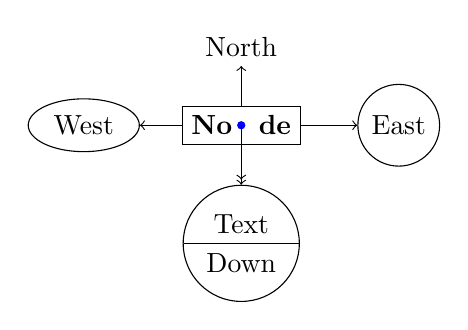
\begin{tikzpicture}
 			\draw (0,0) node(direct)[draw] 
 				{\bf No \, de};
 			\path (0,1) node(nodeNorth) {North};
 			\path (2,0) node(nodeEast)										[draw,shape=circle] {East};
 			% Uses Shapes
 			\path (-2,0) node(nodeWest)  									[draw,shape=ellipse] {West};
 			\draw (0,-1.5) node(split) 
 				[draw, circle split] 
 				{Text \nodepart{lower} Down};
 			%% Drawing Connecting Arrows
 			\fill[blue] (direct) circle (1.5pt);
 			\draw[->] (direct.north) -- (nodeNorth);
 			\draw[->] (direct.east) -- (nodeEast);
 			\draw[->] (direct.west) -- (nodeWest);
 			\draw[->>] (direct.center) -- (split);
 		\end{tikzpicture}
 	\end{figure}
 	
 	\begin{figure}[h]
 		\centering
 		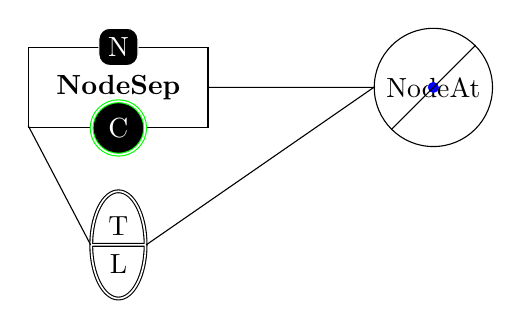
\begin{tikzpicture}
 			\draw (0,0) node(N)[draw, inner sep=10pt] 						{\bf NodeSep};
 			\draw (0,-2) node(ell) 
 				[draw, ellipse split, double]
 				{T \nodepart{lower} L};
 		%% \node[options] (label) at (coord) {content};
 			\node[draw, circle] (nodeAt) at (4,0) 
 				{NodeAt};
 			\node[draw,white,fill=black,rounded corners]
 				at (N.north) {N};
 			\draw (N.east) -- (nodeAt.west) -- 									(ell.east);
 			\fill[blue] (nodeAt.center) circle (2pt);
 			\draw (nodeAt.45) -- (nodeAt.225);
 			\draw (ell.180) -- (N.203);
 			\node[draw,green,fill=black,circle,double]
 				at (N.270) {\textcolor{white}{C}};
 		\end{tikzpicture}
 	\end{figure}
 	
 	\begin{figure}[H]
 		\centering
 		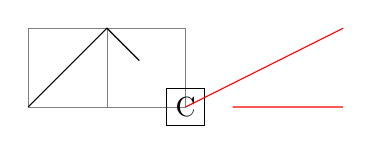
\begin{tikzpicture}
 			\draw[help lines] (0,0) grid (2,1);
 			\coordinate (A) at (0, 0);
			\coordinate (B) at (1, 1);
			\node[draw,outer sep=10pt] (C) at (2,0) {C};
			\draw (A) -- (B) -- (C);
			\draw[red] (C) -- (4,0)
			       	   (2,0) -- (4,1);
 		\end{tikzpicture}
 	\end{figure}
 	
 	\begin{figure}[H]
 		\centering
 		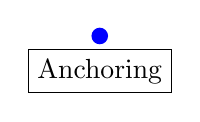
\begin{tikzpicture}
 			\fill[blue] (0,0) coordinate (A) 
 				circle (3pt);
 			\node[draw, anchor=north, outer sep=5pt] at 
 				(A) {Anchoring};
 		\end{tikzpicture}
 	\end{figure}
 	
 	\begin{figure}[H]
 		\centering
 		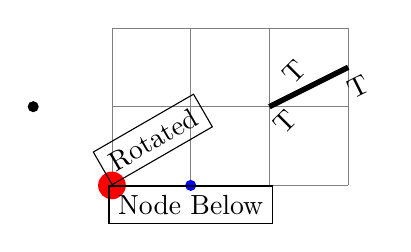
\begin{tikzpicture}
 			\draw[help lines] (0,0) grid (3,2);
 			\coordinate (Sh) at (1,0);
 			\fill[blue] (1,0) coordinate(Sh) 
 				circle (2pt);
 			\fill[red] (0,0) coordinate(A) circle (5pt);
 			\node[draw, below, shift=(Sh)] at (A) 
 				{Node Below};
 			\fill[shift={(-1cm,-1cm)}] (0,2) 
 				circle (2pt);
 			\node[draw, above right, rotate=30] 
 				at (A) {Rotated};
 			%% The pos Option
 			\draw[line width=2pt] (2,1) -- (3,1.5)
 				node[below,rotate=45, pos=0] {T}
 				node[above,rotate=45, midway] {T}
 				node[below, sloped, pos=1] {T};
 		\end{tikzpicture}
 	\end{figure}
 	
 	{\noindent\Large\bf Constructing Trees} \\
 	
 	\begin{figure}[H]
 		\centering
 		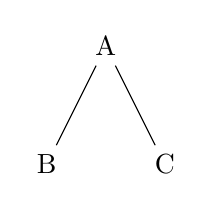
\begin{tikzpicture}
 			\node {A}
 				child{node {B}}
 				child{node {C}};
 		\end{tikzpicture}
 	\end{figure}
 	
 	\begin{figure}[H]
 		\centering
 		\begin{tikzpicture}[
 			every node/.style={draw, circle},
 			level/.style={sibling distance=25mm/#1,
 			level distance=20mm}
 			]
 			\node {A} 
 				child{
					node {B} 
						child{node {$B_1$}}
						child{node {$B_2$}}				
 				}
 				child {
					node {C} 	
						child{node {$C_1$}}
						child{node {$C_1$}}			
 				};
 		\end{tikzpicture}
 	\end{figure}
 	
 	%%%%%%%%%%%%%%%%%%%%%%%%%%%%%%%%%%%%%%%%%%%%%%%%%
 	%%%%%%%%%%%%%%%%%%%%%%%%%%%%%%%%%%%%%%%%%%%%%%%%%
 	\pagebreak
 	
 	\section{Understanding Coordinate Systems}
 	% Explicit (<System> cs: <coord>)
 	% (3,4) = (canvas cs: x=3, y=4)
 	% (x,y,z)
 	\begin{tikzpicture}[>=angle 60, thick, blue]
 		\draw[help lines] (-1,-1) grid (4,2);
 		\draw[->] (0,0) -- (1,0,0) node[anchor=north]
 			{$x$};
 		\draw[->] (0,0) -- (0,1,0) node[anchor=east] 					{$y$};
 		\draw[->] (0,0) -- (0,0,1) 
 			node[anchor=south east] {$z$};
 		%% The Polar System
 		\draw[-stealth, dashed] (0,0) -- (45:1cm);
 		\draw[gray] (0,0) circle (1cm);
 		\draw[-stealth, dashed] (90:2cm) -- (45:1cm);
 		% Changing for the Polar
 		\node[fill, circle, inner sep=1.5pt] (Arc)
 			at (2,0) {};
 		\draw[red] (Arc) -- ++(45:1cm) 
 					(Arc)-- +(125:1.5cm);
 	\end{tikzpicture}
 	\hspace{0.25cm}
 	% The Perp Coord Sys
 	\begin{tikzpicture}
 		\draw[help lines] (0,0) grid (3,3);
 		\node[fill=blue, circle, inner sep=1pt](A) 
			at (1,1) {};
		\node[fill=red, circle, inner sep=1pt](B) 
			at (2,2) {};
		\draw (2,1 -| 1,2) circle (4pt);
		% The Horz and Vert
		\draw (0,1) -- (2,1) (1,0) -- (1,2);
		\draw[dashed] (A |- B) circle (6pt);
		\node[draw] at (A -| B) {};
		\draw[blue] (0,0 -| 0,0) -- (A);
 	\end{tikzpicture}
 	
 	\vspace{0.5cm}
 	
 	\begin{tikzpicture}[scale=1.5, line width=1.5pt]
 		\draw[help lines] (-1,-1) grid (2,2);
 		\fill (0,0,0) circle (1.5pt);
 		% The Blue Path
 		\draw[blue] (0,0,0) -- (0,0,1) -- (0,1,1)
 			-- (0,1,0) -- cycle; % 0 at x for all plane
		\draw[red]  (1,0,0) -- (1,0,1) -- (1,1,1) -- 				(1,1,0) -- cycle; % 1 at x for all plane
		\draw (0,0,0) -- (1,0,0)
			  (0,0,1) -- (1,0,1)
			  (0,1,0) -- (1,1,0)
			  (0,1,1) -- (1,1,1);
 	\end{tikzpicture}
 	
 	\subsection{Relative \& Incremental Coordinates}
 	% The Relative Coordinates
 	\begin{tikzpicture}[thick]
 		\draw[help lines] (0,0) grid (3,3);
 		\draw[blue] (0,0) -- +(1,0)
 					(1,1) -- +(1,1) % (3,2)
 					-- +(2,1) -- +(2,2) -- +(1,1)
 					(0,2) -- +(3,-2); % (3,0)
 	\end{tikzpicture}
 	\hspace{0.25cm}
 	% The Incremental Coordinates
 	\begin{tikzpicture}
 		\draw[help lines] (0,0) grid (3,3);
 		\draw[red] (0,0) -- ++(1,0) % curr (1,0)
 					(1,1) -- ++(1,1) % curr (2,2)
 					-- ++(1,0) -- ++(0,1) -- ++(-2,-1)
 					-- ++(2,-2) -- ++(-3,1);
 	\end{tikzpicture}
 	
 	\vspace{0.5cm}
 	
 	\begin{tikzpicture}
 		\draw[help lines] (0,0) grid +(3,2);
 		\fill       (0,0) circle (1.2pt); 
		\fill[blue] (1,1) circle (1.2pt); 
		\fill[red]  (2,0) circle (1.2pt); 
		%% Absolute Cooredinates
		\draw (0,0) -- (1,0) --
			  (1,1) -- (0,1) -- cycle;
		%% Relative Coordinates 
		\draw[blue] (2,1) -- +(1,0) -- +(1,1) -- +(0,1)
			-- cycle;
		%% Incremental Coordinates
		\draw[red] (2,0) -- ++(1,0) -- ++(0,1) 
			-- ++(-1,0) -- cycle;
		%% Shortcut
		\draw[cyan] (1,1) circle (1pt) % (1,0)
					rectangle ++(1,1);
 	\end{tikzpicture}
 	
 	\vspace{0.3cm}
 	
 	\begin{tikzpicture}[thick]
		\draw[help lines] (0,0) grid +(4,3);
		\fill[blue] (1,2) circle (1.2pt);
		\fill[red]  (3,0) circle (1.2pt);
		%% Absolute Coordinates
		\draw (0,0) -- (1,0) -- (1,1) -- 
				(0,1) -- cycle;
		%% Relative Coordinates
			 % MOVE (2,2)
		\draw[blue] (1,2) -- +(2,-1) -- +(1,1) -- 
				+(1,0) -- cycle;
		%% Incremental Coordinates
			% MOVE (0,2)
		\draw[red] (3,0) -- ++(1,0) -- 
				++(0,1) -- cycle;
	\end{tikzpicture}
	
	%%%%%%%%%%%%%%%%%%%%%%%%%%%%%%%%%%%%%%%%%%%%%%%
	%%%%%%%%%%%%%%%%%%%%%%%%%%%%%%%%%%%%%%%%%%%%%%%
	%%%%%%%%%%%%%%%%%%%%%%%%%%%%%%%%%%%%%%%%%%%%%%%
	
	\section{Defining Styles}
	
	\subsection{By Using the tikzset cmd -- Globally}
	\tikzset{% RDT: red Dashed Triangle
		RDT/.style = {
			fill = red!50, thick, dashed		
		}	
	}
	\begin{tikzpicture}
		\draw[RDT] (0,0) -- (2,0) -- (2,2) -- cycle;
	\end{tikzpicture}
	\hspace{2cm}
	% Defining a Node Style
	\tikzset{% RBN: Round Black Nodes
		RBN/.style = {
			draw, white, fill=black, rounded corners,
			minimum height=0.7cm		
		}
	}
	\begin{tikzpicture}
		% Define the Nodes
		\node[RBN] (left) at (0,0) {Node One};
		\node[RBN] (right) at (2,0) {Node Two};
		% Draw the Arcs
		\draw[-stealth, thick] (left.south) 
			arc(180:360:1 and 0.5);
		\draw[-stealth, thick] (right.north) 
	  		arc(0:180:1 and 0.5);
	\end{tikzpicture}
	
	\subsection{Inserting as a tikzpicture Option}
	\begin{tikzpicture}[
			GDT/.style = {
				fill=green!50, thick, dashed			
			}
		]
		\draw[GDT] (0,0) -- (2,0) -- (2,2) -- cycle;
		%% RDT Still accessible
		\draw[RDT] (3,0) -- (5,0) -- (5,2) -- cycle;
	\end{tikzpicture}
	
	\subsection{Appending to an Existing Style}
	\tikzset{
		RDT/.append style = {
			line width = 2pt	
		}	
	}
	\begin{tikzpicture} % It works as an option too
		\draw[RDT] (0,0) -- (2,0) -- (2,2) -- cycle;
	\end{tikzpicture}
	% Using Arguments
	\hspace{0.5cm}
	\tikzset{
		CRect/.style = {fill=#1, rounded corners},
		CRect/.default = {teal!50}
	}
	\begin{tikzpicture}
		\draw[CRect] (0,0) rectangle (2,2);
		\draw[CRect=cyan!50] (2.5,0) rectangle (4.5,2);
		\draw[CRect=green!50] (5,0) rectangle (7,2);
	\end{tikzpicture}
	% The style 2 args
	\hspace{0.5cm}
	\tikzset{
		Circ/.style 2 args = {
			fill=#1, line width=#2		
		},
		Circ/.default = {brown!50}{1pt}
	}
	\begin{tikzpicture}
		\draw[Circ] (1,1) circle (1);
		\draw[Circ={red!50}{2pt}] (3.5,1) circle (1);
	\end{tikzpicture}
	% Max No. of Args = 9
	\tikzset{
		GBNode/.style n args = {9}{
			draw=#1, fill=#2, inner sep=#3,
			outer sep=#4 ,minimum width=#5,
			minimum height=#6, text=#7, font=#8,
			line width=#9
		}	
	}
	\begin{tikzpicture} 
		\draw[help lines, white] (0,0) grid (7,1);% white grid to serve as a space to allow for placing the node displaced from left.  
    	\node[
    		GBNode=
    		{gray}{black}{3pt}{1pt}{2cm}								{1cm}{white}{\Large\bfseries}{2pt}, 						rounded corners
    		] at (7,0.25) {Node};
	\end{tikzpicture}	
	
	%%%%%%%%%%%%%%%%%%%%%%%%%%%%%%%%%%%%%%%%%%%%%%%%%
	\section{Scopes}
	% Nesting Scopes
	\begin{tikzpicture}[scale=1.5]
	\begin{scope}[fill=red!50]
		\fill[rounded corners] (0,0) rectangle (1,1);
		\begin{scope}[fill=blue!50]
			\fill[rounded corners] 
				(2,0) rectangle (3,1);
		\end{scope}
		\begin{scope}[line width=2pt]
			\filldraw (3.5,0.5) circle (12pt); 
		\end{scope}
		\fill[rounded corners] 
				(4.5,0) rectangle (5.5,1);
	\end{scope}
	\end{tikzpicture} 
	
	\vspace{0.25cm}
	
	\noindent 
	\begin{tikzpicture}[green!50]
		\fill (0,0) circle (1);
		{[fill=red!50]
			\fill (3,0) circle (1);
			{[line width=2pt]
				\filldraw (4.5,0) circle (10pt);
			}
		}
		\fill (6.5,0) circle (1); 
	\end{tikzpicture}
	
	\vspace{0.25cm}
	
	\noindent
	\tikzset{
		scopeStyle/.style={
			fill=blue!50,draw=black,dashed,thick,
			rounded corners
		}
	}
	\begin{tikzpicture}[fill=red!50]
		\fill (0,0) circle (1);
		{
		[scopeStyle]
			\filldraw (3,0) circle (1) 
			  	  (5,-1) rectangle (7,1);		
		}
		\fill (9,0) circle (1);
	\end{tikzpicture}
	
	\section{Repeating Drawings}
	
	\subsection{Using the foreach Command}
	\begin{tikzpicture}[scale=0.5]
		\foreach \r in {1, 2, 3}
			\draw (0,0) circle (\r) 
				  (6.5,0) circle (\r)
				  (0,\r) -- (6.5,\r)
				  (0,-\r) -- (6.5,-\r);
	\end{tikzpicture}
	\hspace{0.5cm}
	\begin{tikzpicture}
		% Reserving a space for the picture 
 		\draw[help lines, white] (0,0) grid (6,2); 
 		\foreach \p in {1,2,3,4}{
 			\fill[teal!80] (\p,2) circle (10pt);
 			\draw[teal!80,thick] (\p,1) circle (10pt); 
 		}
	\end{tikzpicture}
	
	\vspace{0.25cm}
	
	%% Practical example of using polar coord system
	\begin{tikzpicture}
		\draw (0,0) circle (1);
		\foreach \a in {0, 60, 120, 180, 240, 300}{
			\fill (\a:1) circle (0.1);
			\draw (0,0) -- (\a:1);
		}
	\end{tikzpicture}
	
	\vspace{0.25cm}
	
	\begin{tikzpicture}[>=triangle 60]
		\draw[<->,thick] (0,0) -- (8,0);
		\foreach \c in {1,2,...,7}{
			\fill (\c,0) circle (0.1);		
		}
	\end{tikzpicture}
	
	\vspace{0.25cm}
	
	\begin{tikzpicture} 
	 	\draw (0,0) circle (1);
			\foreach \a in {0,30,...,330}{
				\draw (0,0) -- (\a:1);
				\fill (\a:1) circle (0.1);		
			}
 	\end{tikzpicture}
 	
 	\vspace{0.5cm}
 	
 	%% Forms of nested and multi-variable foreach loops
 	\begin{tikzpicture}
 		% 1st:(0x,0y) (0x,1y) | 2nd: (1x,0y) (1x,1y)
 		\foreach \x in {0,1}{
			\foreach \y in {0,1}{
				\draw (\x,\y) circle (10pt);
				\fill (\x,\y) circle (5pt);	
			} 		
 		}
 	\end{tikzpicture}
 	\hspace{0.5cm}
 	\begin{tikzpicture}[line width=2pt]
 		\draw[help lines, white] (0,0) grid (6,2); 
 		\foreach \x/\c in {1/A,2/B,3/C,4/D}{
			\node[draw, circle] at (\x,1) {\c}; 		
 		}
 	\end{tikzpicture}
 	
 	\subsection{Using the pic Command}
 	\tikzset{
		SBR/.pic = {% Small blue rectabgle
			\fill[blue!50] (0,0) rectangle (1,1);
		},
		wheel/.pic = {
			\fill (0.5,0.5) circle (0.4);
			\draw[line width=8pt, line cap=round]
				(0,0) -- (1,1);		
		} 	
 	}
 	\begin{tikzpicture}[
 			rounded corners=2pt,
 			SRR/.pic = {% Small Red Recrangle
				\fill[red!50] (0,0) rectangle (1,1); 	
 			}
 		]
 		\pic at (0,0) {SBR};
 		\pic at (2,0) {SRR};
 		\pic[opacity=0.5] at (4,0) {SRR};
 		\pic at (6,0) {wheel};
 	\end{tikzpicture}
\end{document}